\documentclass[../thesis.tex]{subfiles}
\begin{document}
\section{Experimental Results and Analysis}
\subsection{Test setup}
The benchmark test were performed in three separate scenarios - CPU intensive task on local server, CPU intensive task on remote server and a SELECT database query on local server with a local database setup.
\newline
	
According to one-factor-at-a-time experimental design, we make three fundamental tests - CPU intensive calculation of fibonacci value on local server and remote server, select query to local database in local server. The calculate Fibonacci module calculates some value of Fibonacci and evaluates the performance under compute-intensive tests. Select Operation from local DB module compares different performance through querying some data of DB in an IO-intensive situation. Under all benchmark tests, we keep number of requests at 200 with a concurrency of 1. TABLE 1 summarizes the factors in our experiments.
	
\begin{table}[H]
	\caption{Benchmark test factors}
	\centering
	\footnotesize
	\label{tab1}
	\begin{tabular}{!{\color{sapphire}\vrule width 1pt}m{0.22\textwidth}!{\color{black}\vrule width 1pt}m{0.22\textwidth}!{\color{black}\vrule width 1pt}m{0.22\textwidth}!{\color{black}\vrule width 1pt}m{0.22\textwidth}!{\color{sapphire}\vrule width 1pt}}
		\arrayrulecolor{sapphire}\hline
		\Centering Users &
		\Centering 100, 200, 300, 400, 500 \\
		\hline
		\Centering Requests &
		\Centering 200 \\
		\hline
		\Centering Benchmark test module & 
		\Centering Calculate fibonacci local \& remote server, SELECT query local DB \\
		\hline
		\Centering Web technologies tested & 
		\Centering Node, PHP, Python-Django \\
		\hline
		\arrayrulecolor{sapphire}\hline
	\end{tabular}
\end{table}
In order to achieve fair results, the server machines are rebooted after each test in order to ensure no additional resources are being used up by other running processes or previously running processes.
\newpage
	\begin{figure}[H]
	\centering
	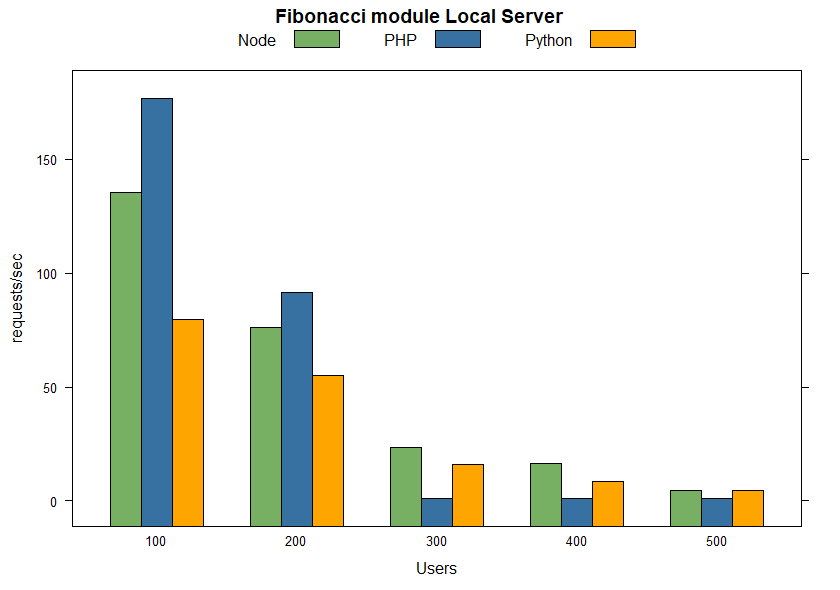
\includegraphics[width=1\textwidth]{../images/fibLocalreq.png}
	\captionsetup{justification=raggedleft, font={it, footnotesize}}
	\captionsetup{justification=justified, font={up, footnotesize}}
	\caption{Throughput, Fibonacci module on local server}
	\label{rys1}
	\end{figure}
			\begin{table}[H]
	\caption{Tabular results for fibonacci module on local server}
	\centering
	\footnotesize
	\label{tab1}
	\bigskip
	\begin{tabular}{!{\color{sapphire}\vrule width 1pt}m{0.22\textwidth}!{\color{black}\vrule width 1pt}m{0.22\textwidth}!{\color{black}\vrule width 1pt}m{0.22\textwidth}!{\color{black}\vrule width 1pt}m{0.22\textwidth}!{\color{sapphire}\vrule width 1pt}}
		\arrayrulecolor{sapphire}\hline
		\Centering \textbf{Users} &
		\Centering \textbf{Node req/sec} &
		\Centering \textbf{PHP req/sec} &
		\Centering \textbf{Python req/sec} \\
		\hline
		\Centering 100 &
		\Centering 135.37 &
		\Centering 176.60 &
		\Centering 79.58 \\
		\hline
		\Centering 200 &
		\Centering 76.06 &
		\Centering 91.72 &
		\Centering 55.18 \\
		\hline
		\Centering 300 &
		\Centering 23.35 &
		\Centering 0.99 &
		\Centering 16.08 \\
		\hline
		\Centering 400 &
		\Centering 16.35 &
		\Centering 0.99 &
		\Centering 8.37 \\
		\hline
		\Centering 500 &
		\Centering 4.70 &
		\Centering 0.89 &
		\Centering 4.64 \\
		\hline
		\arrayrulecolor{sapphire}\hline
	\end{tabular}
\end{table}
\newpage
The graph was obtained by testing the Fibonacci module on the local server machine on the three specified web technologies. It consists of a grouped column chart with the number of Users(requests) on the x-axis and Throughput on the y-axis. The readings are taken at intervals of 100, 200, 300, 400 and 500 users.
\newline

From the graph, we can observe that with the growth of users, the performance of the three technologies shows a decreasing trend. This is expected since as the number of users increases, it increases the load on the server thus slowing down the response time. The throughput is highest in the case of PHP for 100 users with 176.60 requests per second. It is followed by Node which comes in at 135.37 requests per second and then Django at 79.58 requests per second. 
\newline

As the number of users increases there is a downward trend in the value of throughput. At 200 users we observe a similar result with PHP outperforming Node and Django with 91.72 requests per second, Node with 76.06 and Django with 55.18 requests per second.
\newline

However, as we reach the 300 users mark, the result is quite different for the case of PHP. While Node and Django show consistent results, as in decreasing throughput, PHP completely crumbles at this threshold and manages to only get 0.99 requests per second. This suggests that the server is saturated and cannot handle such large number of requests.
With 400 and 500 users we observe a similar situation, with PHP server being completely saturated with 0.99 and 0.89 req/sec respectively, while Node and Django even though have low response rates, have not saturated their servers.
\newpage
\begin{figure}[H]
	\centering
	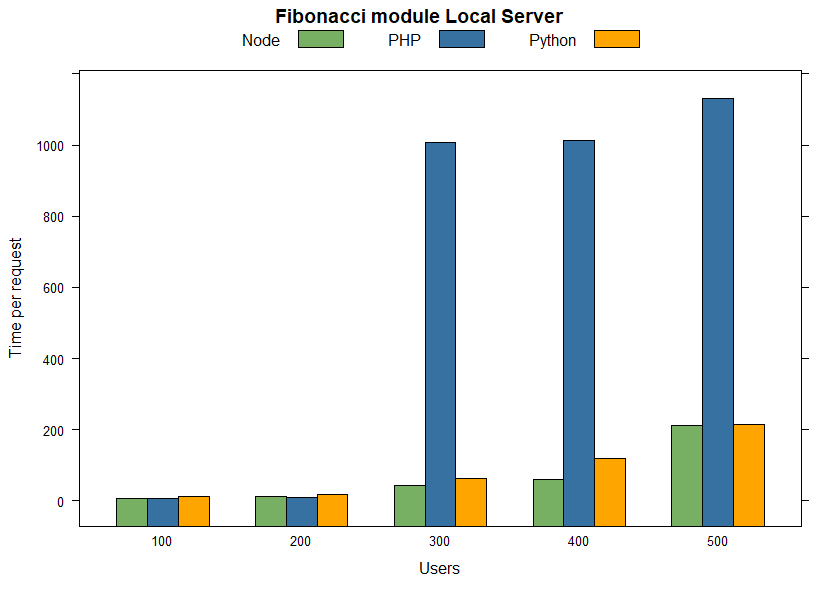
\includegraphics[width=1\textwidth]{../images/fibLocaltpr.png}
	\captionsetup{justification=raggedleft, font={it, footnotesize}}
	\captionsetup{justification=justified, font={up, footnotesize}}
	\caption{Time per request, Fibonacci module on local server}
	\label{rys1}
\end{figure}
\begin{table}[H]
	\caption{Tabular results for fibonacci module on local server}
	\centering
	\footnotesize
	\label{tab1}
	\bigskip
	\begin{tabular}{!{\color{sapphire}\vrule width 1pt}m{0.22\textwidth}!{\color{black}\vrule width 1pt}m{0.22\textwidth}!{\color{black}\vrule width 1pt}m{0.22\textwidth}!{\color{black}\vrule width 1pt}m{0.22\textwidth}!{\color{sapphire}\vrule width 1pt}}
		\arrayrulecolor{sapphire}\hline
		\Centering \textbf{Users} &
		\Centering \textbf{Node} &
		\Centering \textbf{PHP} &
		\Centering \textbf{Python} \\
		\hline
		\Centering 100 &
		\Centering 7.38 ms &
		\Centering 5.66 ms&
		\Centering 12.56 ms\\
		\hline
		\Centering 200 &
		\Centering 13.14 ms&
		\Centering 10.90 ms&
		\Centering 18.12 ms\\
		\hline
		\Centering 300 &
		\Centering 42.83 ms&
		\Centering 1008.46 ms&
		\Centering 62.19 ms\\
		\hline
		\Centering 400 &
		\Centering 61.17 ms&
		\Centering 1011.46 ms&
		\Centering 119.07 ms\\
		\hline
		\Centering 500 &
		\Centering 212.94 ms&
		\Centering 1129.60 ms&
		\Centering 215.63 ms\\
		\hline
		\arrayrulecolor{sapphire}\hline
	\end{tabular}
\end{table}
\newpage
In the above graph we observe the results of the time taken for each request to be completed by testing the Fibonacci module on the local server machine. It consists of a grouped column chart with Users(requests) on the x-axis and time per request on the y-axis.
\newline

From the graph, it is evident that as the number of users increases, the time required to complete each request increases and there is a clear correlation between this graph and the graph for request per second. As the number of users increases, the processing time for each request also increases thus taking more time to complete each request. The time per request is lowest in case of PHP for 100 users with 5.66 ms per request. It is followed by Node with 7.38 ms per request and Python 12.56 ms per request.
\newline

With growing number of users there is a similar observation at 200 users per second with PHP again outperforming Node and Python with 10.90 ms per request against Node's 13.14 and Python's 18.12 ms per request.
\newline

However, as expected from the graph of request per second, when the users is at 300 and beyond, the PHP server gets saturated and the time taken to complete each request skyrockets in comparison to Node and Python which have more consistent results as expected. At this point, PHP takes 1008.46 ms to complete each request which indicates a saturation point in the server, while Node and Python remain unsaturated and clock in times of 42.83 ms and 62.19 ms per request respectively.
\newpage

\begin{figure}[H]
	\centering
	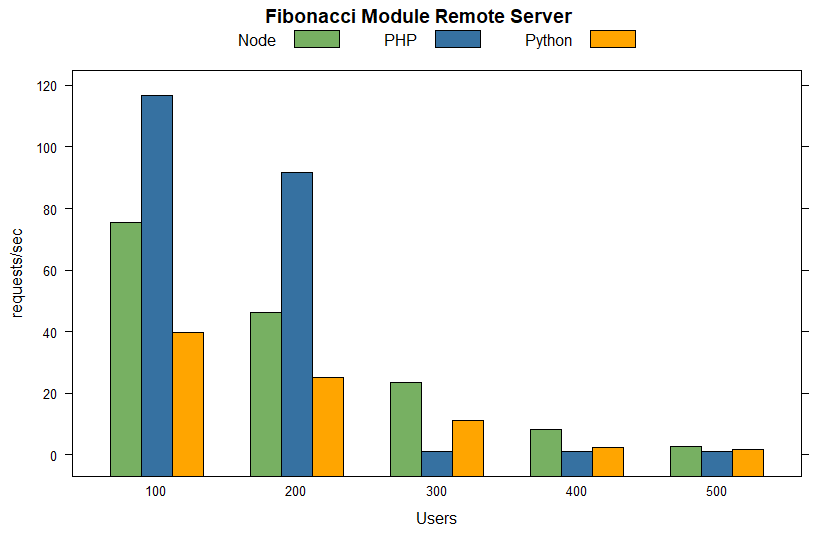
\includegraphics[width=1\textwidth]{../images/fibRemotereq.png}
	\captionsetup{justification=raggedleft, font={it, footnotesize}}
	\captionsetup{justification=justified, font={up, footnotesize}}
	\caption{Throughput, Fibonacci module on remote server}
	\label{rys1}
\end{figure}
\begin{table}[H]
	\caption{Tabular results for fibonacci module on remote server}
	\centering
	\footnotesize
	\label{tab1}
	\bigskip
	\begin{tabular}{!{\color{sapphire}\vrule width 1pt}m{0.22\textwidth}!{\color{black}\vrule width 1pt}m{0.22\textwidth}!{\color{black}\vrule width 1pt}m{0.22\textwidth}!{\color{black}\vrule width 1pt}m{0.22\textwidth}!{\color{sapphire}\vrule width 1pt}}
		\arrayrulecolor{sapphire}\hline
		\Centering \textbf{Users} &
		\Centering \textbf{Node req/sec} &
		\Centering \textbf{PHP req/sec} &
		\Centering \textbf{Python req/sec} \\
		\hline
		\Centering 100 &
		\Centering 75.37 &
		\Centering 116.60 &
		\Centering 39.58 \\
		\hline
		\Centering 200 &
		\Centering 46.06 &
		\Centering 91.72 &
		\Centering 23.23 \\
		\hline
		\Centering 300 &
		\Centering 21.67 &
		\Centering 0.99 &
		\Centering 11.88 \\
		\hline
		\Centering 400 &
		\Centering 8.78 &
		\Centering 0.99 &
		\Centering 2.54 \\
		\hline
		\Centering 500 &
		\Centering 2.76 &
		\Centering 0.99 &
		\Centering 1.49 \\
		\hline
		\arrayrulecolor{sapphire}\hline
	\end{tabular}
\end{table}
\newpage
The graph was obtained by testing the Fibonacci module on the remote server machine hosted on DigitalOcean virtual private network to simulate real-world request type scenario over the Internet. It is a grouped column chart with number of users on x-axis and throughput on the y-axis.
\newline

As seen previously PHP again performs much better when the number of users is relatively low at 100 and 200 users. The graphs shows a similar downtrend as the number of users increases progressively to 500. PHP processes 116.60 requests per second at 100 users while Node comes in at second with 75.37 req/sec and Python with 39.58 requests per second.
A similar result is obtained when the number of users increases to 200 with PHP at 91.72 req/sec, Node 46.06 req/sec and Python at 23.23 req/sec.
\newline

When the number of users increases to 300 and beyond, we obtain a repeat of what we observed with the servers set up on the local machine. The requests processed per second by PHP plummets to 0.99 req/sec indicating signs of saturation while Node and Python maintain their gradual decrease in the number of requests processed per second.
\newline

It is important to note that even though the graph trend on the remote server is very identical to the graphs obtained on the local machine, the overall requests processed per second in the case of the remote server is lower. The most likely cause of this is the bandwidth and distance between the client making the request and the server.
\newpage
	\begin{figure}[H]
	\centering
	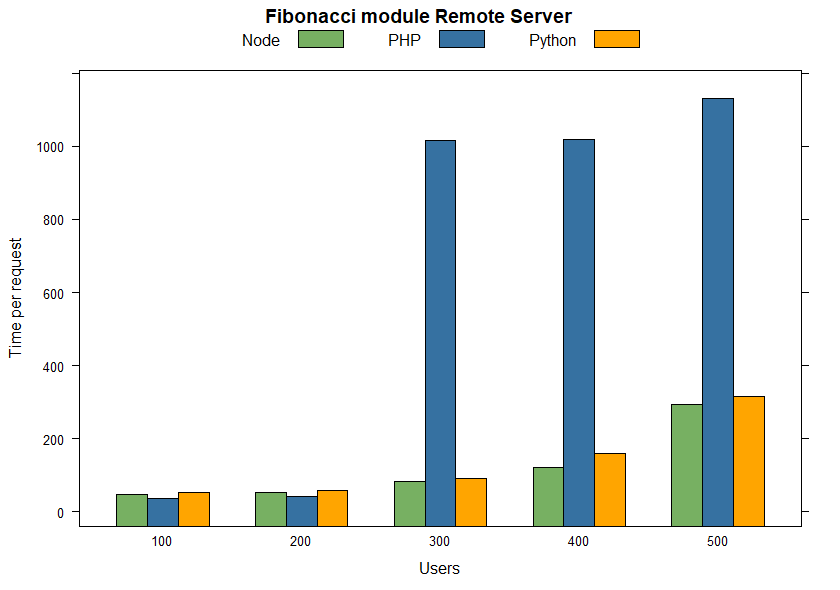
\includegraphics[width=1\textwidth]{../images/fibRemotetpr.png}
	\captionsetup{justification=raggedleft, font={it, footnotesize}}
	\captionsetup{justification=justified, font={up, footnotesize}}
	\caption{Time per request, Fibonacci module on remote server}
	\label{rys1}
\end{figure}
\begin{table}[H]
	\caption{Tabular results for fibonacci module on remote server}
	\centering
	\footnotesize
	\label{tab1}
	\bigskip
	\begin{tabular}{!{\color{sapphire}\vrule width 1pt}m{0.22\textwidth}!{\color{black}\vrule width 1pt}m{0.22\textwidth}!{\color{black}\vrule width 1pt}m{0.22\textwidth}!{\color{black}\vrule width 1pt}m{0.22\textwidth}!{\color{sapphire}\vrule width 1pt}}
		\arrayrulecolor{sapphire}\hline
		\Centering \textbf{Users} &
		\Centering \textbf{Node} &
		\Centering \textbf{PHP} &
		\Centering \textbf{Python} \\
		\hline
		\Centering 100 &
		\Centering 47.23 ms &
		\Centering 35.24 ms&
		\Centering 52.76 ms\\
		\hline
		\Centering 200 &
		\Centering 53.15 ms&
		\Centering 40.84 ms&
		\Centering 58.01 ms\\
		\hline
		\Centering 300 &
		\Centering 82.46 ms&
		\Centering 1015.34 ms&
		\Centering 92.13 ms\\
		\hline
		\Centering 400 &
		\Centering 121.13 ms&
		\Centering 1018.64 ms&
		\Centering 159.12 ms\\
		\hline
		\Centering 500 &
		\Centering 291.41 ms&
		\Centering 1129.14 ms&
		\Centering 315.22 ms\\
		\hline
		\arrayrulecolor{sapphire}\hline
	\end{tabular}
\end{table}
\newpage
The graph was obtained by testing the Fibonacci module on the remote server machine hosted on DigitalOcean virtual private network to simulate real-world request type scenario over the Internet. It is a grouped column chart with number of users on x-axis and time per request (in ms) on the y-axis.
\newline

From the graph, we observe that as in the case with the local server, we obtain similar results. As the number of users increases, the time required to complete each request increases and again there is a clear correlation between this graph and the graph for request per second. As the number of users increases, the processing time for each request also increases thus taking more time to complete each request. The time per request is lowest in case of PHP for 100 users with 35.24 ms per request. It is followed by Node with 47.23 ms per request and Python 52.76 ms per request.
\newline

With growing number of users there is a similar observation at 200 users per second with PHP again outperforming Node and Python with 40.84 ms per request against Node's 53.15 and Python's 58.01 ms per request.
\newline

However, as expected from the graph of request per second, when the users is at 300 and beyond, the PHP server gets saturated and the time taken to complete each request rapidly increases in comparison to Node and Python which have more consistent results as expected. At this point, PHP takes 1015.34 ms to complete each request which indicates a saturation point in the server, while Node and Python remain unsaturated and clock in times of 82.46 ms and 92.13 ms per request respectively.
\newline

We observe that both the cases for request per second and time per request, once the PHP server is saturated there is not much difference in their results. This is an interesting outcome as it indicates that the bandwidth causes a smaller effect on the performance of the server once the server is saturated.
\newpage
\begin{figure}[H]
	\centering
	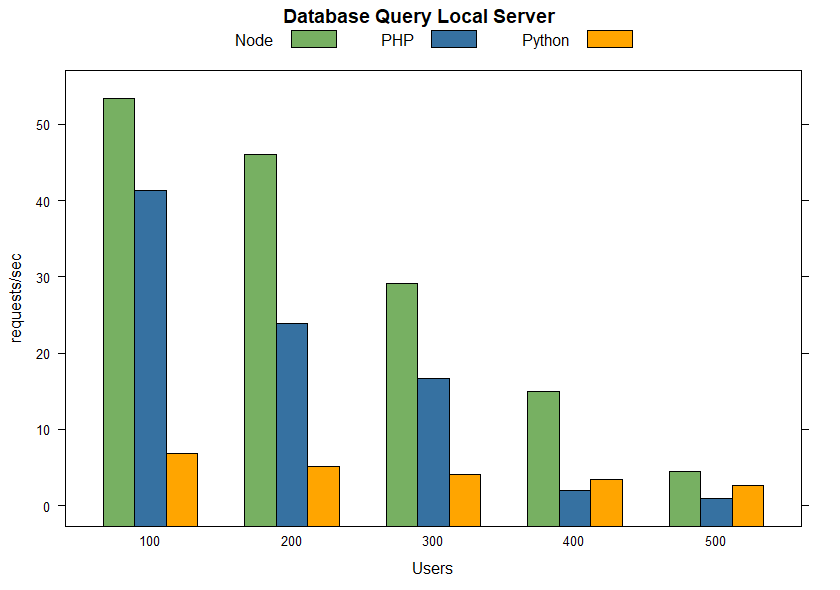
\includegraphics[width=1\textwidth]{../images/dbLocalreq.png}
	\captionsetup{justification=raggedleft, font={it, footnotesize}}
	\captionsetup{justification=justified, font={up, footnotesize}}
	\caption{Throughput, Database query on local server}
	\label{rys1}
\end{figure}
\begin{table}[H]
	\caption{Tabular results for Database query on local server}
	\centering
	\footnotesize
	\label{tab1}
	\bigskip
	\begin{tabular}{!{\color{sapphire}\vrule width 1pt}m{0.22\textwidth}!{\color{black}\vrule width 1pt}m{0.22\textwidth}!{\color{black}\vrule width 1pt}m{0.22\textwidth}!{\color{black}\vrule width 1pt}m{0.22\textwidth}!{\color{sapphire}\vrule width 1pt}}
		\arrayrulecolor{sapphire}\hline
		\Centering \textbf{Users} &
		\Centering \textbf{Node req/sec} &
		\Centering \textbf{PHP req/sec} &
		\Centering \textbf{Python req/sec} \\
		\hline
		\Centering 100 &
		\Centering 53.22 &
		\Centering 41.35 &
		\Centering 6.86 \\
		\hline
		\Centering 200 &
		\Centering 46.06 &
		\Centering 23.83 &
		\Centering 5.12 \\
		\hline
		\Centering 300 &
		\Centering 29.18 &
		\Centering 16.07 &
		\Centering 4.10 \\
		\hline
		\Centering 400 &
		\Centering 14.99 &
		\Centering 1.96 &
		\Centering 3.42 \\
		\hline
		\Centering 500 &
		\Centering 4.5 &
		\Centering 0.89 &
		\Centering 2.52 \\
		\hline
		\arrayrulecolor{sapphire}\hline
	\end{tabular}
\end{table}
\newpage
The graph was obtained by testing the database query on the local server machine on the three specified web technologies. It consists of a grouped column chart with the number of Users(requests) on the x-axis and throughput on the y-axis. The data is stored in a relational database using PostgreSQL.
\newline

We obtain a very interesting result in this test. Unlike the previous results on the fibonacci module, PHP does not perform as well as it did previously. We observe a more consistent result among all the three technologies at least up until 300 users. Node performs the best out of the three with 52.22 req/sec at 100 users followed by PHP at 41.35 req/sec and then Python with 6.86 req/sec. A similar trend is observed at 200 and 300 users with each technology showing consistently decreasing results.
\newline

However, at 400 and beyond, the PHP server again saturates, causing a drop in the throughput, even below that of Python's. At 400 users, Node comes in at 14.99 req/sec with Python in second at 3.42 req/sec and then PHP with 1.96 req/sec. There is a drastic fall in the req/sec processed by PHP indicating that the server has saturated.
\newline

What we observe in the three technologies in this scenario is that Node performs better in an I/O intensive operation rather than a CPU intensive operation. PHP is able to handle more users before reaching it's saturation point in case of I/O operations, but once it reaches saturation, it again drop to ~ 1 req/sec range. Python overall has considerably low throughput value, indicating that it may not be the best option for I/O operations, however, it still shows consistent readings and does not reach saturation as easily as PHP does.
\newpage
\begin{figure}[H]
	\centering
	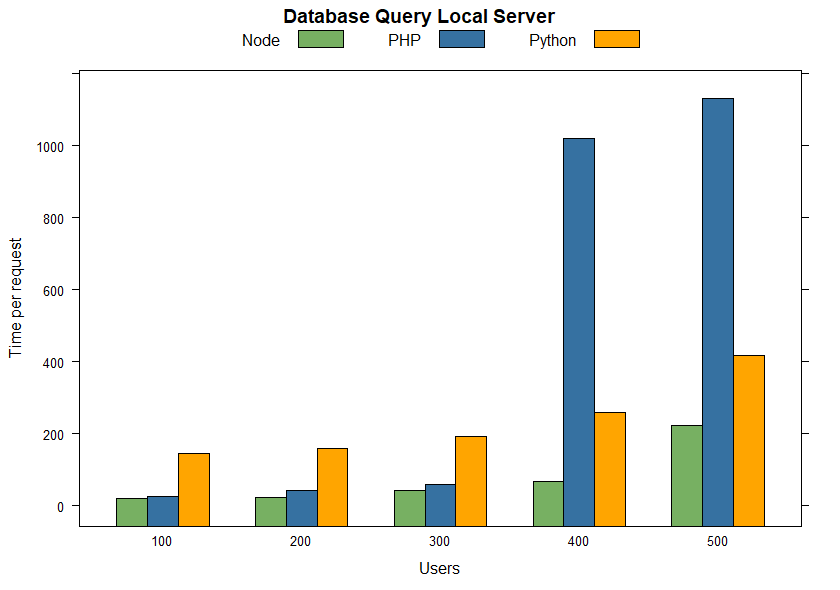
\includegraphics[width=1\textwidth]{../images/dbLocaltpr.png}
	\captionsetup{justification=raggedleft, font={it, footnotesize}}
	\captionsetup{justification=justified, font={up, footnotesize}}
	\caption{Time per request, Database query on local server}
	\label{rys1}
\end{figure}
\begin{table}[H]
	\caption{Tabular results for fibonacci module on remote server}
	\centering
	\footnotesize
	\label{tab1}
	\bigskip
	\begin{tabular}{!{\color{sapphire}\vrule width 1pt}m{0.22\textwidth}!{\color{black}\vrule width 1pt}m{0.22\textwidth}!{\color{black}\vrule width 1pt}m{0.22\textwidth}!{\color{black}\vrule width 1pt}m{0.22\textwidth}!{\color{sapphire}\vrule width 1pt}}
		\arrayrulecolor{sapphire}\hline
		\Centering \textbf{Users} &
		\Centering \textbf{Node} &
		\Centering \textbf{PHP} &
		\Centering \textbf{Python} \\
		\hline
		\Centering 100 &
		\Centering 18.74 ms &
		\Centering 24.20 ms&
		\Centering 145.86 ms\\
		\hline
		\Centering 200 &
		\Centering 21.51 ms&
		\Centering 41.43 ms&
		\Centering 158.12 ms\\
		\hline
		\Centering 300 &
		\Centering 42.83 ms&
		\Centering 59.54 ms&
		\Centering 192.42 ms\\
		\hline
		\Centering 400 &
		\Centering 66.70 ms&
		\Centering 1018.46 ms&
		\Centering 259.24 ms\\
		\hline
		\Centering 500 &
		\Centering 222.94 ms&
		\Centering 1129.60 ms&
		\Centering 415.23 ms\\
		\hline
		\arrayrulecolor{sapphire}\hline
	\end{tabular}
\end{table}
\newpage
The graph was obtained by testing the database query on the local server machine on the three specified web technologies. It consists of a grouped column chart with the number of Users(requests) on the x-axis and time per request on the y-axis. The data is stored in a relational database using PostgreSQL.
\newline

As seen in the above test for database query of users vs. req/sec, we observe a strong correlation between the two graphs. Node has the lowest time taken to complete a request coming in at 18.74 ms per request followed by PHP at 24.20 ms per request and eventually Python at 145.86 ms per request.
\newline

At 400 and beyond, the PHP server again saturates, causing a spike in the time per request, even over that of Python's. At 400 users, Node comes in at 66.70 ms per request with Python in second at 259.24 ms per request and then PHP with 1018.46 ms per request. There is a drastic increase in the time per request processed by PHP indicating that the server has saturated.
\newline

\newpage
\end{document}